\documentclass[11pt, a4paper]{article}

% 한글 지원 (XeLaTeX)
\usepackage{fontspec}
\setmainfont{Noto Sans CJK KR}
\setsansfont{Noto Sans CJK KR}
\setmonofont{Noto Sans CJK KR}

% 컬러 이모지 (Twitter Emoji)
\usepackage{twemojis}

% 페이지 설정
\usepackage[margin=2cm]{geometry}
\usepackage{setspace}
\onehalfspacing

% 이미지
\usepackage{graphicx}

% 색상
\usepackage{xcolor}
\definecolor{mainblue}{HTML}{1565C0}
\definecolor{applegreen}{HTML}{43A047}
\definecolor{honeyyellow}{HTML}{FFC107}
\definecolor{warmcream}{HTML}{FFFBF5}
\definecolor{textdark}{HTML}{3E2723}
\definecolor{textmedium}{HTML}{5D4037}
\definecolor{bordercolor}{HTML}{FFCCBC}
\definecolor{blueprimary}{HTML}{1976D2}

% 표
\usepackage{array}
\usepackage{booktabs}
\usepackage{tabularx}
\usepackage{colortbl}
\usepackage{multirow}

% 박스 및 프레임
\usepackage{tcolorbox}
\tcbuselibrary{skins, breakable}

% 목록
\usepackage{enumitem}
\setlist[itemize]{leftmargin=*, noitemsep, topsep=3pt}
\setlist[enumerate]{leftmargin=*, noitemsep, topsep=3pt}

% 하이퍼링크
\usepackage{hyperref}
\hypersetup{
    colorlinks=true,
    linkcolor=mainblue,
    urlcolor=blueprimary
}

% 코드/verbatim
\usepackage{listings}
\lstset{
    basicstyle=\ttfamily\small,
    backgroundcolor=\color{warmcream},
    frame=single,
    rulecolor=\color{bordercolor},
    breaklines=true
}

% 헤더/푸터
\usepackage{fancyhdr}
\pagestyle{fancy}
\fancyhf{}
\fancyhead[L]{\small\color{textmedium}사과 가격 예측 시뮬레이터 퀵가이드}
\fancyhead[R]{\small\color{textmedium}v1.2.4.4}
\fancyfoot[C]{\thepage}
\renewcommand{\headrulewidth}{0.5pt}

% 섹션 스타일
\usepackage{titlesec}
\titleformat{\section}
    {\Large\bfseries\color{mainblue}}
    {\thesection}{1em}{}
\titleformat{\subsection}
    {\large\bfseries\color{textdark}}
    {\thesubsection}{1em}{}
\titleformat{\subsubsection}
    {\normalsize\bfseries\color{textmedium}}
    {\thesubsubsection}{1em}{}

% tcolorbox 스타일 정의
\newtcolorbox{infobox}[1][]{
    colback=warmcream,
    colframe=mainblue,
    fonttitle=\bfseries,
    title=#1,
    boxrule=1pt,
    arc=4pt
}

\newtcolorbox{successbox}[1][]{
    colback=green!5,
    colframe=applegreen,
    fonttitle=\bfseries,
    title=#1,
    boxrule=1pt,
    arc=4pt
}

\newtcolorbox{warningbox}[1][]{
    colback=yellow!5,
    colframe=honeyyellow!80!black,
    fonttitle=\bfseries,
    title=#1,
    boxrule=1pt,
    arc=4pt
}

\newtcolorbox{tipbox}{
    colback=blue!5,
    colframe=blueprimary,
    boxrule=0.5pt,
    arc=4pt,
    left=5pt, right=5pt, top=5pt, bottom=5pt
}

% 수식
\usepackage{amsmath}
\usepackage{amssymb}

% 문서 시작
\begin{document}

% 제목 페이지
\begin{center}
    {\Huge\bfseries\color{mainblue} \texttwemoji{red apple} 사과 가격 예측 시뮬레이터}\\[0.5cm]
    {\LARGE\bfseries 퀵가이드}\\[1cm]
    {\large 당도와 무게로 계산된 \textbf{품질 점수}로 사과 가격을 예측해보세요!}\\[1cm]
    \colorbox{mainblue}{\color{white}\bfseries\large\ \ v1.2.4.4\ \ }\\[1.5cm]
\end{center}

\tableofcontents
\newpage

%==============================================================================
\section{\texttwemoji{open book} 이 문서 사용법}
%==============================================================================

\begin{infobox}[이 퀵가이드는 시뮬레이터 옆에 띄워두는 '내비게이션'입니다]
시뮬레이터를 조작하면서 동시에 참조하는 용도로 제작되었습니다.
\end{infobox}

\subsection{권장 사용 방법}

\begin{itemize}
    \item \textbf{화면 분할}: 시뮬레이터 70\% + 퀵가이드 30\%
    \item \textbf{별도 기기}: PC에서 시뮬레이터, 태블릿에서 퀵가이드
    \item \textbf{인쇄}: A4 양면 인쇄하여 실습 시 참조
\end{itemize}

\subsection{상황별 활용법}

\begin{center}
\begin{tabular}{ll}
    \toprule
    \textbf{상황} & \textbf{참조 섹션} \\
    \midrule
    처음 시작 & 1분 초속성 실습 (2절) \\
    버튼 위치 모름 & 화면 구성 (6절) \\
    용어가 헷갈림 & 핵심 용어 (11절) \\
    관찰 방법 모름 & 이런 장면을 찾아보세요 (5절) \\
    문제 발생 & 도와주세요! 선이 이상해요 (9절) \\
    심화 학습 & 문서 읽기 순서 (3절) \\
    \bottomrule
\end{tabular}
\end{center}

%==============================================================================
\section{\texttwemoji{high voltage} 1분 초속성 실습}
%==============================================================================

\begin{successbox}[지금 바로 해보세요!]
가이드를 읽기 전에 먼저 성공 경험을 맛보세요.
\end{successbox}

\vspace{0.5cm}

\begin{center}
\begin{tabular}{clcc}
    \toprule
    \textbf{단계} & \textbf{행동} & \textbf{확인} & \\
    \midrule
    \textbf{1} & \colorbox{mainblue}{\color{white}\small\ 데이터 생성\ } 버튼 클릭 & 점들이 나타났나요? & $\square$ \\[3pt]
    \textbf{2} & \colorbox{applegreen}{\color{white}\small\ 학습 실행\ } 버튼 클릭 & 빨간 선이 그려졌나요? & $\square$ \\[3pt]
    \textbf{3} & R$^2$ 점수 확인 & \textbf{0.9 이상}이면 성공! & $\square$ \\
    \bottomrule
\end{tabular}
\end{center}

\vspace{0.5cm}

\begin{tipbox}
\textbf{Tip:} 성공했다면 이제 아래 내용을 읽으며 \textbf{왜} 그렇게 되었는지 알아보세요!
\end{tipbox}

%==============================================================================
\section{\texttwemoji{books} 문서 읽기 순서}
%==============================================================================

더 깊이 알고 싶다면 아래 순서대로 학습하세요.

\vspace{0.3cm}

\begin{center}
\begin{tabular}{clccl}
    \toprule
    \textbf{순서} & \textbf{문서} & \textbf{소요시간} & \textbf{대상} & \textbf{설명} \\
    \midrule
    1 & \textbf{퀵가이드} (현재) & 10분 & 모두 & 빠른 시작, 핵심 기능 \\
    2 & 사용설명서 & 20분 & 모두 & 전체 기능 상세 설명 \\
    3 & 이론해설서 & 30분 & 모두 & 선형 회귀 이론 학습 \\
    4 & 활용가이드 & 20분 & 교사 & 수업 활용 방법 \\
    5 & 수업지도안 & 15분 & 교사 & 차시별 수업 계획 \\
    \bottomrule
\end{tabular}
\end{center}

%==============================================================================
\section{\texttwemoji{eyes} 한눈에 보기}
%==============================================================================

\begin{center}
\begin{tabular}{lp{10cm}}
    \toprule
    \textbf{항목} & \textbf{내용} \\
    \midrule
    목적 & 선형 회귀로 사과 가격 예측 학습 \\
    입력 변수 & 당도(Brix), 무게(g) $\rightarrow$ \textbf{품질 점수} \\
    출력 & 예측 가격(원) \\
    핵심 개념 & 가중치, 편향, 경사 하강법, R$^2$ 점수, 오차(잔차) \\
    그래프 & \textbf{X축: 품질, Y축: 가격} (단순 선형 회귀) \\
    \bottomrule
\end{tabular}
\end{center}

%==============================================================================
\section{\texttwemoji{magnifying glass tilted left} 이런 장면을 찾아보세요!}
%==============================================================================

\begin{infobox}[{단순히 보지 말고, 관찰하세요}]
아래 현상이 보이면 학습이 잘 되고 있는 것입니다!
\end{infobox}

\subsection{학습 중 관찰 포인트}

\begin{center}
\begin{tabular}{lp{6cm}l}
    \toprule
    \textbf{관찰 대상} & \textbf{찾아볼 장면} & \textbf{의미} \\
    \midrule
    손실 그래프 & `L'자로 급격히 꺾이며 내려가나요? & 빠르게 학습 중 \\
    회귀선 & 점들의 중심을 관통하나요? & 패턴을 잘 찾는 중 \\
    R$^2$ 점수 & 0에서 1로 가까워지나요? & 정확도 상승 중 \\
    \bottomrule
\end{tabular}
\end{center}

\subsection{오차선 관찰 포인트}

\begin{center}
\begin{tabular}{lp{6cm}l}
    \toprule
    \textbf{관찰 대상} & \textbf{찾아볼 장면} & \textbf{의미} \\
    \midrule
    오차선 길이 & 대부분 짧아졌나요? & 예측이 정확해짐 \\
    오차선 색상 & 빨강 $\rightarrow$ 녹색으로 변했나요? & 오차가 줄어듦 \\
    긴 오차선 & 유독 긴 선이 있나요? & 이상치(Outlier) \\
    \bottomrule
\end{tabular}
\end{center}

\begin{tipbox}
\textbf{분석가의 눈:} ``왜 저 점은 오차가 클까?'' 생각해보세요!
\end{tipbox}

%==============================================================================
\section{\texttwemoji{desktop computer} 화면 구성}
%==============================================================================

\subsection{학습 모드}

\begin{center}
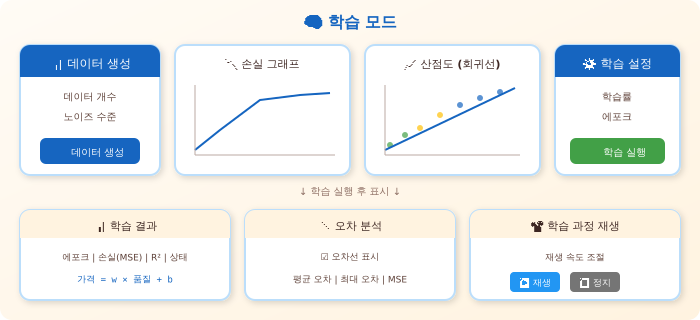
\includegraphics[width=0.95\textwidth]{퀵가이드_06_학습모드화면구성_v1.0.0.0_초안작성_2026-02-01_1721.png}
\end{center}

\subsection{추론 모드}

\begin{center}
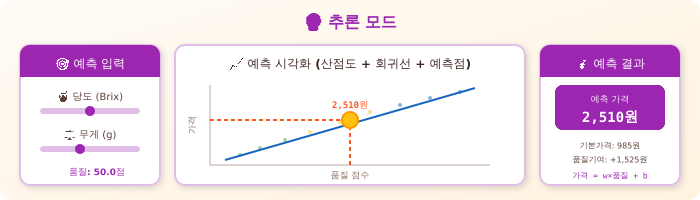
\includegraphics[width=0.95\textwidth]{퀵가이드_06_추론모드화면구성_v1.0.0.0_초안작성_2026-02-01_1721.png}
\end{center}

%==============================================================================
\section{\texttwemoji{triangular ruler} 품질 점수 계산}
%==============================================================================

당도와 무게를 \textbf{하나의 품질 점수}로 통합합니다:

\begin{tcolorbox}[colback=warmcream, colframe=bordercolor]
\begin{center}
\textbf{품질 = 당도점수(50\%) + 무게점수(50\%)}
\end{center}

\begin{align*}
\text{당도점수} &= \frac{\text{당도} - 10}{8} \times 50 \quad \text{(10--18 Brix에서 0--50점)} \\[0.3cm]
\text{무게점수} &= \frac{\text{무게} - 150}{200} \times 50 \quad \text{(150--350g에서 0--50점)}
\end{align*}

\textbf{예시:} 당도 14 Brix인 경우 $(14-10)/8 \times 50 = 25$점
\end{tcolorbox}

%==============================================================================
\section{\texttwemoji{gear} 주요 파라미터}
%==============================================================================

\begin{center}
\begin{tabular}{lcp{7cm}}
    \toprule
    \textbf{파라미터} & \textbf{권장값} & \textbf{설명} \\
    \midrule
    데이터 개수 & 20--50개 & 너무 적으면 과적합, 많으면 느림 \\
    노이즈 & 10\% & 실제 데이터의 불확실성 표현 \\
    학습률 & 0.01 & 너무 크면 발산, 작으면 느림 \\
    에포크 & 500회 & 손실이 안정되는 시점까지 \\
    \bottomrule
\end{tabular}
\end{center}

%==============================================================================
\section{\texttwemoji{sos} 도와주세요! 선이 이상해요}
%==============================================================================

\begin{warningbox}[문제가 생겼나요?]
아래에서 증상을 찾아보세요.
\end{warningbox}

\vspace{0.3cm}

\begin{center}
\begin{tabular}{llp{5cm}}
    \toprule
    \textbf{증상} & \textbf{원인} & \textbf{해결책} \\
    \midrule
    선이 춤을 춰요 & 학습률 높음 & 학습률을 \textbf{0.01 이하}로 \\
    선이 안 움직여요 & 학습률 낮음 & 학습률을 높이거나 재생 속도 올리기 \\
    손실이 안 줄어요 & 학습률 부적절 & 초기화 후 0.01로 재시도 \\
    선이 화면 밖으로 & 학습 발산 & 학습률을 \textbf{0.001}로 \\
    R$^2$가 음수 & 학습 부족 & 에포크 늘리기 또는 데이터 늘리기 \\
    추론 모드 작동 안 함 & 학습 안 됨 & 학습 모드에서 먼저 학습 \\
    \bottomrule
\end{tabular}
\end{center}

%==============================================================================
\section{\texttwemoji{question} 자주 묻는 질문}
%==============================================================================

\subsection{데이터 관련}

\textbf{Q: 데이터를 몇 개 생성해야 하나요?}\\
A: 처음에는 20--30개로 시작하세요. 5개 미만은 불안정, 100개는 복잡합니다.

\vspace{0.3cm}

\textbf{Q: 노이즈는 왜 있나요?}\\
A: 실제 데이터는 완벽하지 않습니다. 같은 품질의 사과도 가격이 다를 수 있습니다.

\subsection{학습 관련}

\textbf{Q: 손실 그래프가 올라갔다 내려갔다 해요}\\
A: 학습률이 너무 큽니다. 0.01 이하로 낮춰보세요.

\vspace{0.3cm}

\textbf{Q: 학습할 때마다 결과가 달라요}\\
A: 정상입니다! 초기값이 랜덤이지만, 충분히 학습하면 비슷한 결과에 도달합니다.

%==============================================================================
\section{\texttwemoji{key} 핵심 용어}
%==============================================================================

\begin{center}
\small
\begin{tabular}{llp{4cm}p{4cm}}
    \toprule
    \textbf{용어} & \textbf{학술 용어} & \textbf{의미} & \textbf{쉬운 설명} \\
    \midrule
    품질 점수 & Feature & 당도+무게 통합 점수 & 사과의 종합 점수 \\
    가중치 & Weight, Slope & 영향력 (기울기) & 품질 1점은 가격 몇 원? \\
    편향 & Bias, Intercept & 기본값 (절편) & 품질 무관 기본 가격 \\
    손실 & Loss, MSE & 예측과 실제의 차이 & AI가 얼마나 틀렸는지 \\
    오차선 & Residual & 실제값-예측값 & 틀린 정도 시각화 \\
    학습률 & Learning Rate & 업데이트 크기 & 한 걸음에 얼마나 배울지 \\
    에포크 & Epoch & 전체 학습 횟수 & 데이터를 몇 번 볼지 \\
    R$^2$ 점수 & Coef. of Determination & 모델 적합도 (0--1) & 모델이 얼마나 잘 맞는지 \\
    회귀선 & Regression Line & 관계를 나타내는 직선 & 예측을 위한 직선 \\
    \bottomrule
\end{tabular}
\end{center}

\vspace{0.5cm}

\begin{tipbox}
\textbf{수학 시간에 배운 $y = ax + b$ 기억나세요?}\\
여기서 $a$가 기울기(가중치), $b$가 절편(편향)입니다!
\end{tipbox}

%==============================================================================
\section{\texttwemoji{trophy} 나의 베스트 R$^2$ 기록}
%==============================================================================

\begin{center}
\begin{tabular}{cccccc}
    \toprule
    \textbf{시도} & \textbf{데이터 수} & \textbf{노이즈} & \textbf{학습률} & \textbf{에포크} & \textbf{R$^2$ 점수} \\
    \midrule
    1 & \hspace{1.5cm} & \hspace{1.2cm} & \hspace{1.2cm} & \hspace{1.2cm} & \hspace{1.5cm} \\[0.5cm]
    2 & & & & & \\[0.5cm]
    3 & & & & & \\[0.5cm]
    \midrule
    \textbf{최고 기록} & & & & & \\[0.3cm]
    \bottomrule
\end{tabular}
\end{center}

\vspace{0.5cm}

\begin{center}
\textbf{도전 목표: R$^2$ > 0.95 달성해보세요!}
\end{center}

%==============================================================================
\section{\texttwemoji{thought balloon} 생각해보기}
%==============================================================================

\begin{tcolorbox}[colback=blue!5, colframe=blueprimary, boxrule=1pt]
\begin{center}
\textbf{\large 이 AI가 예측한 가격이 실제 시장 가격과 다르다면,\\[0.3cm]
누구의 책임일까요?}\\[0.5cm]
\textit{데이터의 문제일까요? 모델의 문제일까요?\\
아니면 세상이 그만큼 복잡한 걸까요?}
\end{center}
\end{tcolorbox}

%==============================================================================
\section{\texttwemoji{file folder} 파일 정보}
%==============================================================================

\begin{center}
\begin{tabular}{lp{10cm}}
    \toprule
    \textbf{항목} & \textbf{내용} \\
    \midrule
    파일명 & 사과가격예측\_선형회귀\_시뮬레이터\_v1.2.4.1.html \\
    실행 방법 & 웹 브라우저에서 열기 \\
    권장 브라우저 & Chrome, Edge, Firefox \\
    \bottomrule
\end{tabular}
\end{center}

%==============================================================================
% 문서 정보
%==============================================================================
\vfill
\begin{center}
\rule{0.8\textwidth}{0.5pt}\\[0.3cm]
{\small\color{textmedium}
사과 가격 예측 시뮬레이터 퀵가이드 v1.2.4.4\\
2026-02-01\\
청주교육대학교 컴퓨팅사고 및 AI교육
}
\end{center}

\end{document}
